\documentclass[preprint,12pt]{elsarticle}

    \usepackage[sc]{mathpazo} % Use the Palatino font
    \usepackage[T1]{fontenc} % Use 8-bit encoding that has 256 glyphs
    \usepackage{microtype} % Slightly tweak font spacing for aesthetics
    \usepackage[english]{babel} % Language hyphenation and typographical rules
    \usepackage{booktabs} % Horizontal rules in tables
    \usepackage{enumitem} % Customized lists
    \usepackage[table,xcdraw]{xcolor}
    \usepackage[utf8]{inputenc} % Required for inputting international characters
    \usepackage{parskip}
    \usepackage{graphicx}
    \usepackage{hyperref}
    \usepackage{pdfpages}
    \usepackage{amsmath}
    \usepackage{esvect}
    \usepackage{listings}
    \usepackage{color}
    \usepackage{spverbatim}
    \usepackage{subcaption}
    \usepackage[title]{appendix}
    \hypersetup{
        colorlinks=true,
        linkcolor=blue,
        filecolor=magenta,      
        urlcolor=cyan,
    }
    \definecolor{dkgreen}{rgb}{0,0.6,0}
    \definecolor{gray}{rgb}{0.5,0.5,0.5}
    \definecolor{mauve}{rgb}{0.58,0,0.82}
    \definecolor{lightgray}{rgb}{0.83, 0.83, 0.83}
    \definecolor{timberwolf}{rgb}{0.86, 0.84, 0.82}
    \definecolor{whitesmoke}{rgb}{0.96, 0.96, 0.96}
    
    \lstset{frame=tb,
    language=python,
    aboveskip=3mm,
    belowskip=3mm,
    showstringspaces=false,
    columns=flexible,
    basicstyle={\small\ttfamily},
    numbers=none,
    numberstyle=\tiny\color{gray},
    keywordstyle=\color{blue},
    commentstyle=\color{dkgreen},
    stringstyle=\color{mauve},
    breaklines=true,
    breakatwhitespace=true,
    tabsize=3,
    backgroundcolor = \color{whitesmoke}
    }

    \begin{document}
    \title{\LARGE \bf
        STAT 391 Homework 4
        }
        
        \author{ \parbox{3 in}{\centering Chongyi Xu \\
                 University of Washington\\
                 STAT 391 Spring 2018\\
                 {\tt\small chongyix@uw.edu}}
        }
    \maketitle

    \section{Problem 1 - Rescuing Rob}
    \begin{enumerate}[label=\alph*]
        \item Estimate the parameters $\mu$ and $\sigma^2$ of the 
        normal density that best fits the data in the file hw4-ugrad.dat
        by the Maximum Likelihood method.\\

        The Maximum Likelihood estimation basiclly calculate for 
        the mean and the variance of the given data $\mathbb{X}$ and 
        use the sample mean as $\mu$ and the sample variance as $\sigma^2$

        \begin{lstlisting}
from statistics import *

# Read in files
# a) hw4-ugrad.dat
dir = r'C:\Users\johnn\Documents\UW\SchoolWorks\2018Spring\STAT391\HW4'
f = open(dir+r'\hw4-ugrad.dat')

x = [float(xx) for xx in f.readline().split(' ')]

# ML mu is the mean of data
mu = mean(x)

# ML sigma is the variance of the data
sigma = stdev(x)

print('The estimated mu is ', mu)
print('And the estimated sigma^2 is ', sigma**2)
        \end{lstlisting}

        And the result I got is 
        \begin{spverbatim}
The estimated mu is  10.018379536
And the estimated sigma^2 is  1.029920746065191
        \end{spverbatim}

        \item Estimate the parameters $a,b$ of the logistic density
        that best fits the data in the file hw4-boiler.dat by the
        Maximum Likelihood method. Make a plot of the log-likelihood
        of the data at each iteration.\\

        From lecture notes (6.24), we obtained the log-likelihood
        of the logistic density distribution,

        \begin{equation*}
            l(a,b) = nln(a) - a\sum_{i}x_i - nb - 2\sum_{i} ln(1+e^{-ax_i-b})
        \end{equation*}

        And therefore, the partial derivatives with respecting to $a,b$  are
        \begin{align*}
            \frac{\partial l}{\partial a} &= \frac{n}{a} - \sum_{i} x_i\frac{1-e^{-ax_i-b}}{1+e^{-ax_i-b}}\\
            \frac{\partial l}{\partial b} &= -\sum_{i} \frac{1-e^{-ax_i-b}}{1+e^{-ax_i-b}}
        \end{align*}

        Since the system is not able to solved analytically, we have to guess for the 
        solution by gradient ascent. The estimated $\hat{a},\hat{b}$ are 
        \begin{align*}
            \hat{a} &\leftarrow \tilde{a} + \eta \frac{\partial l}{\partial a}\\
            \hat{b} &\leftarrow \tilde{b} + \eta \frac{\partial l}{\partial b}
        \end{align*}
        where $\tilde{a}=1$ and $\tilde{b}=0$ are the intial guess for $a,b$.

        \begin{lstlisting}
# b) hw4-boiler.dat
f = open(dir+r'\hw4-boiler.dat')

xb = [float(xx) for xx in f.readline().split(' ')]

step = 0.000001
n = len(xb)
iterations = 50000
ll = [0.0]*(iterations-1)
a = [0.0]*iterations
b = [0.0]*iterations
tol = 0.00001
a[0] = 1

def ll_logistic(a, b, x, n):
    return n*np.log(a) - a*sum(x) - n*b - \
            2*sum(np.log(1 + np.exp([-a*xi-b for xi in x])))
def grad_a(a, b, x, n):
    return n/a - sum([xi*(1-np.exp(-a*xi-b))\
                    /(1+np.exp(-a*xi-b)) for xi in x])
def grad_b(a, b, x):
    return -sum((1-np.exp([-a*xi-b for xi in x]))\
                    /(1+np.exp([-a*xi-b for xi in x])))

for i in range(iterations-1):
    ll[i] = ll_logistic(a[i], b[i], xb, n)
    ga = grad_a(a[i], b[i], xb, n)
    gb = grad_b(a[i], b[i], xb)
    if (abs(ga) < tol and abs(gb) < tol):
        break
    a[i+1] = a[i] + step*ga
    b[i+1] = b[i] + step*gb
    
index,=np.where(np.array(ll)==max(ll))
ll = ll[0:index[0]+1]
a_ML = a[index[0]]
b_ML = b[index[0]]
print('The index is ', index[0])
print('The estimated a is ', a_ML)
print('The estimated b is ', b_ML)

plt.figure(1)
plt.plot(np.arange(index[0]+1), ll)
plt.title('Log-likelihood')
plt.xlabel('Iteration')
plt.show()

plt.figure(2)
plt.plot(a,b, 'o', Linewidth=0.8)
plt.title('Parameters a,b')
plt.xlabel('a')
plt.ylabel('b')
plt.show()

        \end{lstlisting}

        \begin{figure}[htbp!]
            \center
            \begin{subfigure}{0.8\textwidth}
                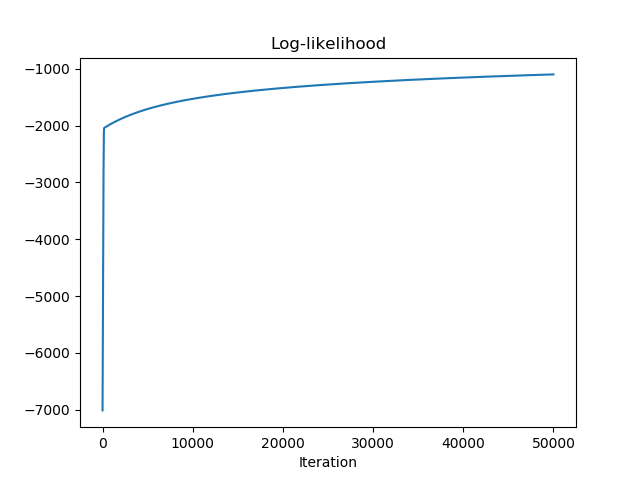
\includegraphics[width = \textwidth]{1.png}
                \caption{The Log-likelihood of the data}
                \label{fig:11}
            \end{subfigure}
            \begin{subfigure}{0.8\textwidth}
                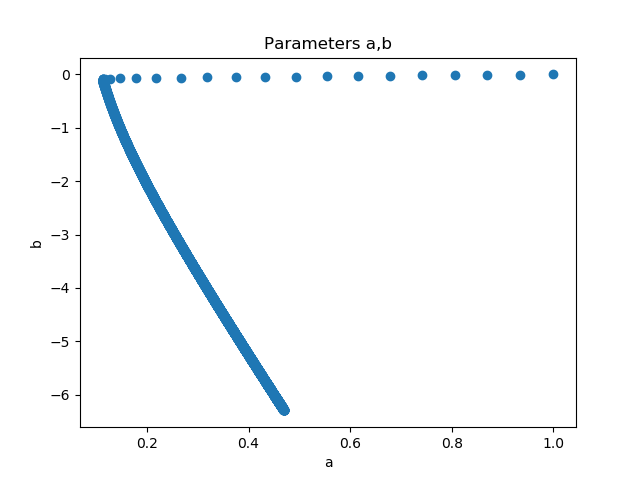
\includegraphics[width = \textwidth]{2.png}
                \caption{The values of paramter $a,b$}
                \label{fig:12}
            \end{subfigure}
            \caption{Estimation of logistic density}
            \label{fig:1}
        \end{figure}
        And the plot is Figure \ref{fig:1}.\\

        And since we are expecting the Maximum Likelihood estimation of 
        $\hat{a},\hat{b}$ are $arg max ll(x;a,b)$. And the iteration method
        will be guaranteed to converge to a local maximum of the log-likelihood,
        therefore, the $a,b$ are
        \begin{lstlisting}
i,=np.where(np.array(ll)==max(ll))
a_ML = a[i[0]]
b_ML = b[i[0]]
print('The estimated a is ', a_ML)
print('The estimated b is ', b_ML)
        \end{lstlisting}

        \begin{spverbatim}
a_ML = 0.142120071559142
b_ML = -1.992443901848966 
        \end{spverbatim}

        \item Compute a kernel density estimate for the data in the file
        hw4-coke.dat using a Gaussian kernel with kernel width $h=0.5$.\\

        Since we are using a Gaussian kernel, then
        \begin{align*}
            k(x) &= \frac{1}{\sqrt{2\pi}}e^{-\frac{x^2}{2}}\\
            \Rightarrow f_X(x) &= \frac{1}{nh}\sum_{i=1}^n k(\frac{x-x_i}{h}) \\
            &= \frac{1}{500\cdot 0.5}\sum_{i} \frac{1}{\sqrt{2\pi}} exp(\frac{(-\frac{x-x_i}{h})^2}{2})\\
            &= \frac{1}{250\sqrt{2\pi}}\sum_{i} e^{-2(x-x_i)^2}
        \end{align*}

        \begin{lstlisting}
# c). hw4-coke.dat
f = open(dir+r'\hw4-coke.dat')
h = 0.5
xc = [float(xx) for xx in f.readline().split(' ')]
n = len(xc)
        \end{lstlisting}

        \item After having had his memory restored, Rob suddenly finds himself
        facing an unknown object whose signature is given in the file hw4-unknown.dat.
        Help Rob once more: tell him what is the object in front of him.\\

        \begin{lstlisting}
# d). hw4-unknown.dat
f = open(dir+r'\hw4-unknown.dat')

x_test = [float(xx) for xx in f.readline().split(' ')]

classes = ['People', 'Furniture', 'Trash']
score = [0]*len(classes)
score[classes.index('People')] = sum(np.log(norm.pdf(x_test, mu, sigma)))
score[classes.index('Furniture')] = sum([np.log(a_ML*np.exp(-a_ML*xi-b_ML)/\
                                        (1+np.exp(-a_ML*xi-b_ML))) for xi in x_test])
for xi in x_test:
    score[classes.index('Trash')] += np.log(1/(n*h)*sum(1/math.sqrt(2*math.pi)*\
                                    np.exp([-(xi-xci)**2/(2*(h**2)) for xci in xc])))
    
print('The Log-Likelihood Score for People is ', score[classes.index('People')])
print('The Log-Likelihood Score for Furniture is ', score[classes.index('Furniture')])
print('The Log-Likelihood Score for Trash is ', score[classes.index('Trash')])
print('The Best Score is ', classes[score.index(max(score))], ' with ', max(score))
        \end{lstlisting}
        \begin{spverbatim}
The Log-Likelihood Score for People is  -485.12788083461237
The Log-Likelihood Score for Furniture is  -791.6883358525606
The Log-Likelihood Score for Trash is  -1018.3103894355676
The Best Score is  Furniture  with  -485.12788083461237s
        \end{spverbatim}

        Therefore, the unknown object should be people.

        \item Make a plot of the densities evaluated in a,b,c and of the data
        $D_{unknown}$ on the same graph.

        \begin{figure}[htbp!]
            \center
            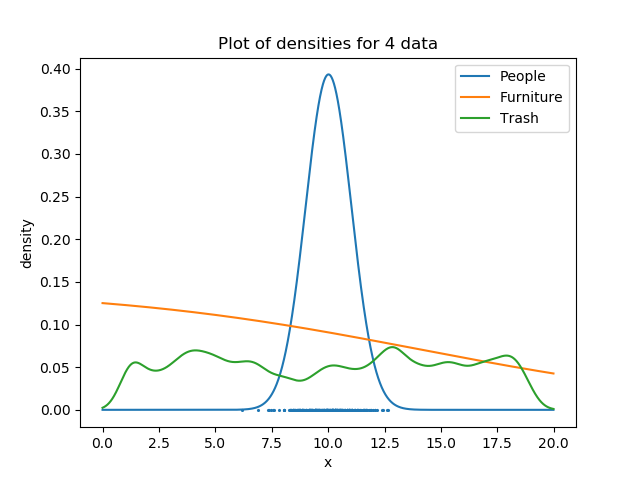
\includegraphics[width = 0.8\textwidth]{3.png}
            \caption{Plot of densities for People, Furniture, Trash.
            The scatter points are the unknown object, we can see
            that the scatter points follows the normal distribution
            pretty well}
            \label{fig:2}
        \end{figure}

        The plot is Figure\ref{fig:2}.
    \end{enumerate}

    \section{Problem 2 - Maximum Likelihood with censored data}
    \begin{enumerate}[label=\alph*]
        \item Write the probability that $y_i=1$ as a function of $\gamma$.
        \begin{equation*}
            P(y_i=1) = P(x_i>1) = 1 - P(x_i<1) = 1 - (1-e^{-\gamma})=e^{-\gamma}
        \end{equation*}

        \item Derive the expression of the log=likelihood $l(\gamma)=ln P(y_i:n||\gamma)$
        as a function of $\gamma$
        \begin{align*}
            l(\gamma) &= ln P(y_i:n|\gamma) \\
                &= ln[(e^{-\gamma})^{\sum_{i}y_i}(1-e^{-\gamma})^{n-\sum_{i}y_i}]\\
                &= ln(e^{-\gamma})\sum_{i}y_i + ln(1-e^{-\gamma})(n-\sum_{i}y_i)
        \end{align*}

        \item Maximize $l$ with respecting to $\gamma$ and obtain the expression for
        $\gamma^{ML}$.\\
        Denote $\theta=e^{-\gamma}$. Then $l(\theta) = ln(\theta)\sum_{i}y_i + ln(1-\theta)(n-\sum_{i}y_i)$.
        \begin{align*}
            \frac{\partial l}{\partial \theta} &= \frac{\sum_{i}y_i}{\theta} - (n-\sum_{i}y_i)\frac{1}{1-\theta} = 0\\
            0 &= (1-\theta)\sum y_i - (n-\sum y_i)\theta \\
            0 &= \sum y_i - n\theta\\
            \theta &= \frac{\sum y_i}{n}\\
            \Rightarrow \gamma^{ML} &= -ln(\frac{\sum y_i}{n})
        \end{align*}

        \item Does this problem have sufficient statistics? How many and what are they?\\

        There is only one sufficient statistics in this problem which is the mean of $y_i$.

        \item Is the estimate of $\gamma$ you are obtaining "bettter", "worse", "the same"
        as you would have obtained had you not lost the original data $x_{1:n}$?\\

        I think that the estimation should be better than using the original data. Since 
        using this method is determing if the output is greater than 1. Comparing to original
        data, $y_i$ will be less varied which will have less variance. In the other words, 
        it will give a "better" result. The "better" generally means less varied centering at
        the "real" $\gamma$

        \item Sample $n=100$ points from an exponential distribution with $\gamma=1$, 
        censor them, and estimate $\gamma^{ML}$ from $x_{1:n}$ and $\gamma^c$ from 
        $y_{1:n}$. Compare the accuracy of the values obtained.

        \begin{lstlisting}
import numpy as np
import matplotlib.pyplot as plt
sample_size = 100
np.random.seed(123)
N = 10000
gammaML = [0.0]*N
gammaC = [0.0]*N

for i in range(N):
    x = np.random.exponential(1, sample_size)
    y = (x>1).astype(int)
    gammaML[i] = sample_size/sum(x)
    gammaC[i] = -np.log(sum(y)/sample_size)

plt.figure(1)
plt.hist(gammaC, bins=30, edgecolor='black')
plt.title('Histogram of gamma^c')
plt.xlabel('gamma^c')
plt.show()

plt.figure(2)
plt.hist(gammaML, bins=30, edgecolor='black')
plt.title('Histogram of gamma^ML')
plt.xlabel('gamma^ML')
plt.show()
        \end{lstlisting}
        \begin{figure}[htbp!]
            \center
            \begin{subfigure}{0.8\textwidth}
                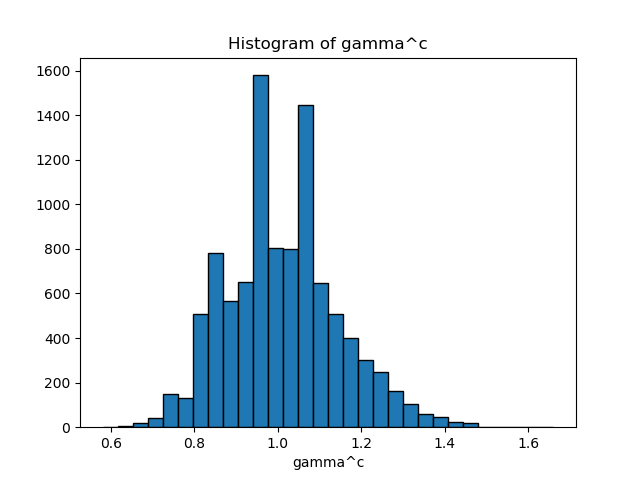
\includegraphics[width = \textwidth]{4.png}
                \caption{The histogram of $\gamma^c$}
                \label{fig:31}
            \end{subfigure}
            \begin{subfigure}{0.8\textwidth}
                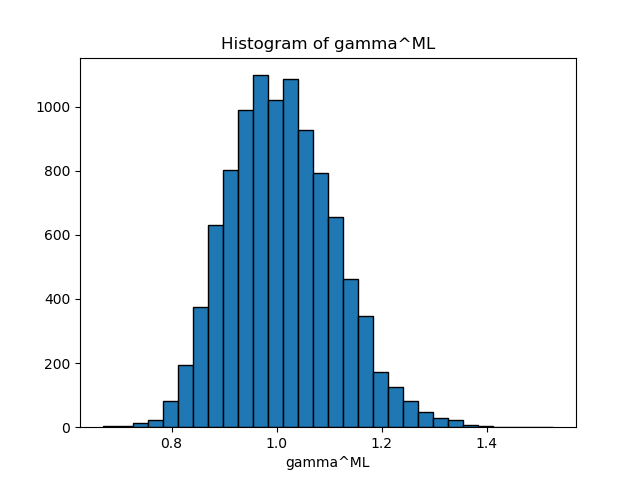
\includegraphics[width = \textwidth]{5.png}
                \caption{The histogram of $\gamma^{ML}$}
                \label{fig:32}
            \end{subfigure}
            \caption{From the figure, we can see both centering at $\gamma=1$, but 
            $\gamma^{ML}$ is generally less varied rather than $\gamma^c$.}
            \label{fig:3}
        \end{figure}

        The figure is Figure\ref{fig:3}
    \end{enumerate}

    \section{Estimating h by cross-validation}
    \begin{enumerate}[label=\alph*]
        \item Read in the training set $D$ consisting of $n = 1000$ samples from F and 
        validation set $D_v$ of m = 300 samples from files hw4-f-train.dat, hw4-f-valid.dat. 
        Use a kernel of your choice and then find the optimal kernel width h by 
        cross-validation. Repeat this for several values of h and plot $L_v(h)$ and $L(h)$ as a
        function of h on the same graph.\\
        Let $h^{*}$ be the $h$ that maximizes $L_v(h)$. Make a plot of $f_{h^{*}}(x)$. Plot
        the true $f(x)$ on the same graph.

        For this question, I will choose the kernel function to be Gaussian function
        \begin{equation*}
            k(x) = \frac{1}{\sqrt{2\pi}}e^{-x^2/2}
        \end{equation*}
        Therefore, my $f_h(x)$ will be 
        \begin{equation*}
            f_h(x) = \frac{1}{nh}\sum_{i} \frac{1}{sqrt{2\pi}}e^{\frac{-(x-x_i)^2}{2h^2}}
        \end{equation*}
        \begin{lstlisting}
import numpy as np
import math 
import matplotlib.pyplot as plt

def findLL(train, test, h):
    ll = [0.]*len(test)
    n = len(train)
    for i in range(len(test)):
        ll[i] = np.log(1/(n*h)*sum(1/math.sqrt(2*math.pi)*\
                    np.exp([-(test[i] - xi_train)**2/(2*h**2) \
                        for xi_train in train])))
    return ll


dir = r'C:\Users\johnn\Documents\UW\SchoolWorks\2018Spring\STAT391\HW4'
f = open(dir+r'\hw4-f-train.dat')
train = [float(xx) for xx in f]

f = open(dir+r'\hw4-f-valid.dat')
valid = [float(xx) for xx in f]

h = [0.001, 0.002, 0.005, 0.01, 0.02, 0.05, 0.1, 0.2, 0.5]
Lv = [0.]*len(h)
L = [0.]*len(h)

for k in range(len(h)):
    Lv[k] = sum(findLL(train, valid, h[k]))
    L[k] = sum(findLL(train, train, h[k]))

plt.figure(1)
plt.plot(h, Lv, label='Lv(h)')
plt.plot(h, L, label='L(h)')
plt.title('The likelihood of the data in D_v under f_h')
plt.xlabel('h')
plt.legend()
plt.show()

hmax = h[np.where(Lv==max(Lv))[0][0]]
x = np.arange(-0.5, 1.5, 0.01)
fx = np.array([0.]*len(x))
fx[np.logical_and(x<=1, x>=0)] = 2 * x[np.logical_and(x<=1, x>=0)]
plt.figure(2)
plt.plot(x, np.exp(findLL(train, x, hmax)), label='f_h(x)')
plt.plot(x, fx, label='f(x)')
plt.xlabel('x')
plt.title('f(x) and f_h(x) at h* = %f'% hmax)
plt.legend()
plt.show()
        \end{lstlisting}
        \begin{figure}[htbp!]
            \center
            \begin{subfigure}{0.8\textwidth}
                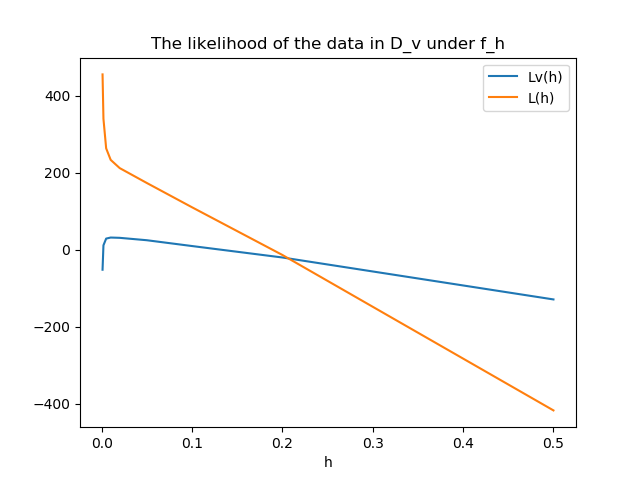
\includegraphics[width = \textwidth]{6.png}
                \caption{The likelihood $L_v(x)$ of the data in $D_v$ and 
                $L(x)$ of the data in training set $D$}
                \label{fig:41}
            \end{subfigure}
            \begin{subfigure}{0.8\textwidth}
                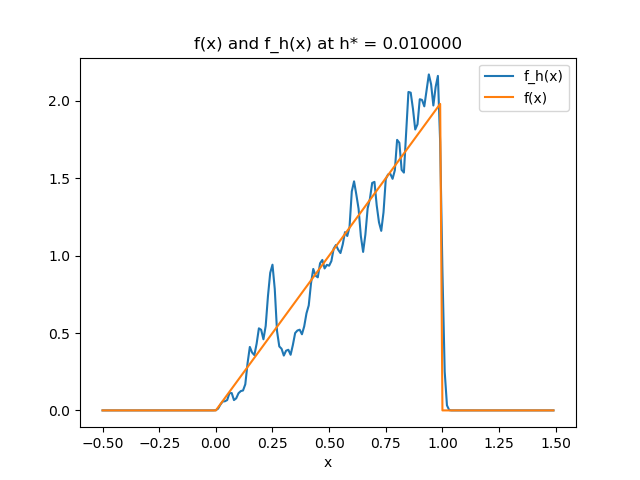
\includegraphics[width = \textwidth]{7.png}
                \caption{$f_h^{*}(x)$ with real $f(x)$ at $h^{*} = 0.01$}
                \label{fig:42}
            \end{subfigure}
            \caption{The plot shows that the kernel density at $h^{*}$ is 
            pretty close to the real $f(x)$}
            \label{fig:4}
        \end{figure}
        The Figure\ref{fig:4} shows the result. As a result, $h^{*}$ I found is 
        \begin{spverbatim}
        >>> h[np.where(Lv==max(Lv))[0][0]]
        0.01
        \end{spverbatim}

        \item Same for $G$ and $g$ from the files hw4-g-train.dat, hw4-g-valid.dat.\\

        Basically same code as I did in part (a) with slight changes
        \begin{lstlisting}
dir = r'C:\Users\johnn\Documents\UW\SchoolWorks\2018Spring\STAT391\HW4'
f = open(dir+r'\hw4-g-train.dat')
train = [float(xx) for xx in f]

f = open(dir+r'\hw4-g-valid.dat')
valid = [float(xx) for xx in f]

h = [0.001, 0.002, 0.005, 0.01, 0.02, 0.05, 0.1, 0.2, 0.5]
Lv = [0.]*len(h)
L = [0.]*len(h)

for k in range(len(h)):
    Lv[k] = sum(findLL(train, valid, h[k]))
    L[k] = sum(findLL(train, train, h[k]))

plt.figure(1)
plt.plot(h, Lv, label='Lv(h)')
plt.plot(h, L, label='L(h)')
plt.title('The likelihood of the data in D_v under g_h')
plt.xlabel('h')
plt.legend()
plt.show()

hmax = h[np.where(Lv==max(Lv))[0][0]]
x = np.arange(-0.5, 1.5, 0.01)
gx = np.array([0.]*len(x))
for i in range(len(x)):
    if x[i]>=0 and x[i]<=0.5:
        gx[i] = 4*x[i]
    elif x[i]>=0.5 and x[i]<= 1:
        gx[i] = 4*(1-x[i])

plt.figure(2)
plt.plot(x, np.exp(findLL(train, x, hmax)), label='g_h(x)')
plt.plot(x, gx, label='g(x)')
plt.xlabel('x')
plt.title('g(x) and g_h(x) at h* = %f'% hmax)
plt.legend()
plt.show()
        \end{lstlisting}
        \begin{figure}[htbp!]
            \center
            \begin{subfigure}{0.8\textwidth}
                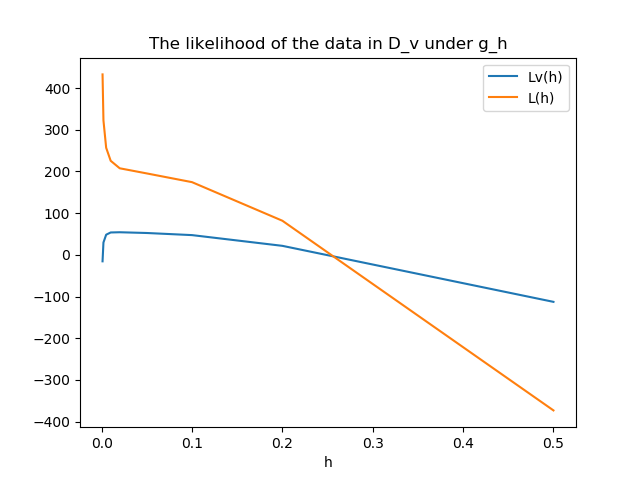
\includegraphics[width = \textwidth]{8.png}
                \caption{The likelihood $L_v(x)$ of the data in $D_v$ and 
                $L(x)$ of the data in training set $D$}
                \label{fig:51}
            \end{subfigure}
            \begin{subfigure}{0.8\textwidth}
                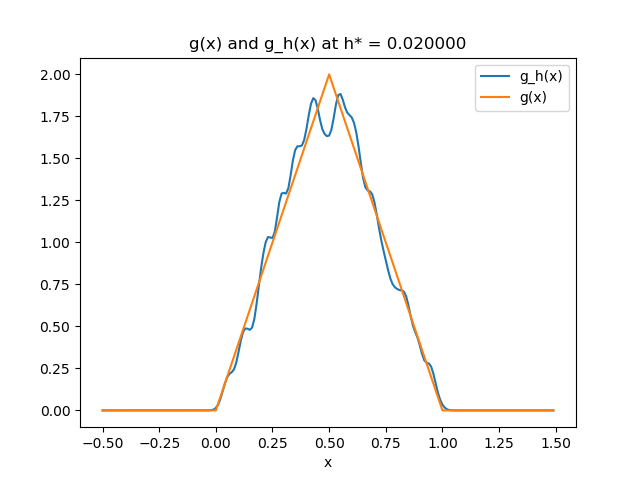
\includegraphics[width = \textwidth]{9.png}
                \caption{$g_h^{*}(x)$ with real $g(x)$ at $h^{*} = 0.02$}
                \label{fig:52}
            \end{subfigure}
            \caption{The plot shows that the kernel density at $h^{*}$ is 
            pretty close to the real $g(x)$, even better than what we have
            for $f(x)$.}
            \label{fig:5}
        \end{figure}
        The plot is Figure\ref{fig:5} and the $h^{*}$ we have for $g(x)$ is 
        \begin{spverbatim}
>>> h[np.where(Lv==max(Lv))[0][0]]
0.02
        \end{spverbatim}

        \item Compare the optimal h's and the quality of the plots in a,b. Which 
        of the densities looks easier to approximate? Which of the optimal kernels 
        widths is larger?\\
        
        From our result, we find out that $g(x)$ is somehow easier to approxiate 
        rather than $y(x)$. And the optimal kernel width for $g(x)$ is larger than 
        $y(x)$. The reason might be that for larger width the variance of esimated
        density will be less.

    \end{enumerate}

\end{document}